\documentclass[12pt,letterpaper]{article}
\usepackage{preamble}

\newcommand\course{MS108}
\newcommand\userID{518030910440}
\setcounter{section}{0}
\begin{document}
%\textbf{\Large RISC-V Report}
\section{Abstract}
    This is a report of the project of MS108 homework implementing a simplified CPU supporting some of the RISC-V instruction sets. 
    My solution is based on Tomasulo algorithm. 
\section{Feature}
\subsection{Tomasulo}
    The Tomasulo algorithm aims to execute Out-of-Order(abbreviated OoO), 
    and solve problems triggered by OoO, such as WAR, WAW, and so on. The key is renaming, 
    RS and ROB. 

    In my design, each FU has its own RS, and the size of each RS is different. 
    Renaming is based on where the instruction is in ROB. 
\subsection{Cache}
    I implemented a 512B I-cache in my project, then I made it a 2-way associative one, but there is little improvement. 
    I guess this is because the testbench only contains short codes. 

    I've also implemented a D-cache with writing back. This performs well in simulation, 
    but costs a great amount of logic units(20\% more LUT) so I give up. 

    My 2-way associative cache and D-cache are in /backup/Units. 
\subsection{Branch Policy}
    I first designed one without branch prediction and its policy is stall. Since branch instructions hold about sixth of instructions, 
    this one stalls frequently and is not so OoO. 

    Then I made one with branch prediction. Like BOOM(Berkeley OoO Machine), it uses shadow registers and branch masks. 
    Each instruction has a branch mask to evidence if it follows in-flight branch instructions. After executing a branch instruction, 
    it boardcasts to update others' branch masks. Only Execute load/store instructions without branch mask. 
    
    Branch prediction policy is simply GShare, and this one can run at 100MHz. 

    This sounds cool, but when I implemented it, I found the delay high, since to deal with the boardcast of branch instructions, 
    a large number of logic units are needed. (let alone the shadow registers cost considerable sources too)

    But it runs faster and is really COOOOOOOOL. 
\section{Summary}
    1. The main problem I face is not understanding how improve in organization and hardware level. 
    Once I noticed that I had repeated calculating one same thing in each RS, so I picked it out: 
    calculate it outside and send the result to each RS. 

    The result was crazy: the number of LUT increased considerably. 

    2. The Tomasulo is significantly efficient when handling a set of load/store instructions. 

    3. The greatest creation is executing some instructions the moment it enters ROB, instead of waiting until 
    the next clock(which is the moment ready becomes 1). 10\% faster. 

    4. The biggest drawbck is unsupporting some kinds of precise exceptions, as it does not handle branch misprediction in ROB. 

    This is easy to fix: simply making all results of Load/Store/Branch instructions enter the ROB with free branch mask 
    and commit them is OK. 

    Other can-be improvements include superscalar, superpipeline and some design details, 
    such as how to get an instruction from RAM in only 4 cycles(can called prefetch), 
    how to write faster(write buffer), how to calculate faster(distributed ALUs and a big mux) etc.. 
\section{Reference}
1. \url{https://docs.boom-core.org/en/latest/}, an out of order RISC-V CPU using chisel, with branch bits(named branch mask there)

2. \url{http://www.kroening.com/diplom/diplom/main003.html}, details about the hardware of Tomasulo Architecture.
\section{Design}
\begin{figure}[H]
    \centering
    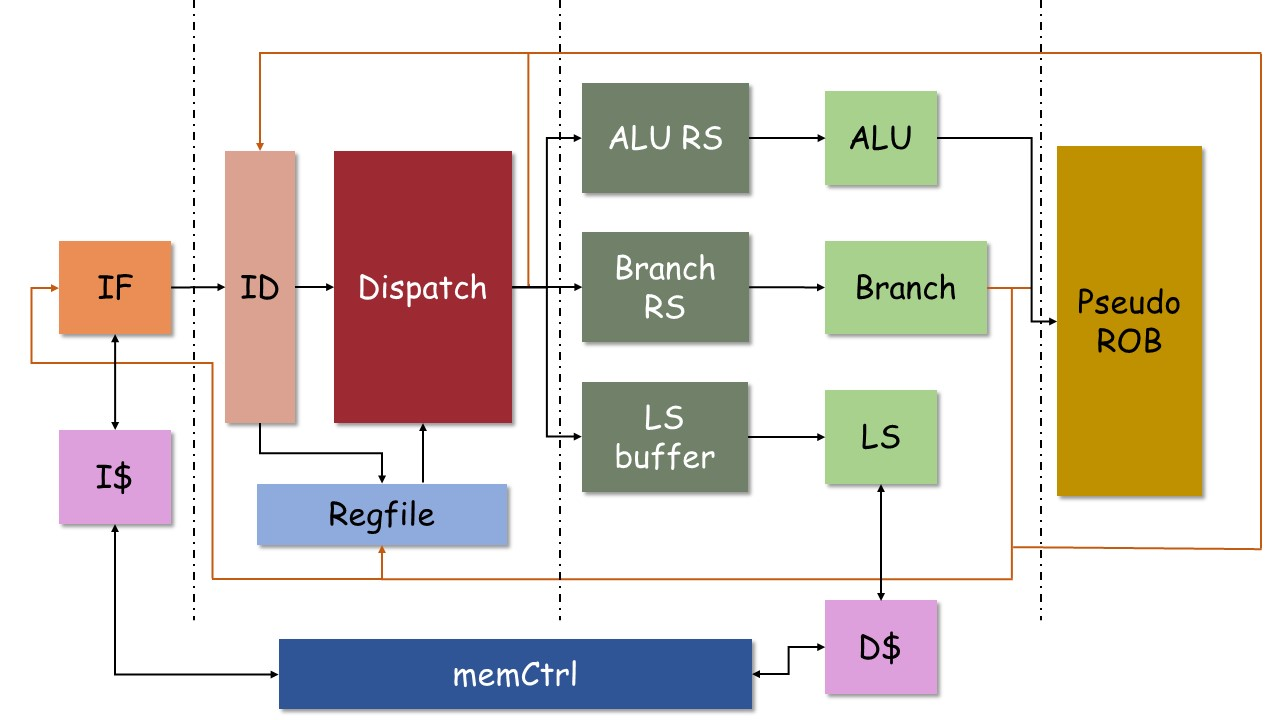
\includegraphics[width=165mm]{design.jpg}
\end{figure}
\end{document}